\subsection{Model Performance Overview}
\label{subsec:pmc-results-model-performance-overview}

This section evaluates the ability of regression models to estimate peak memory usage from shape parameters.
Given the earlier evidence of near-linear scaling with volume, the primary focus is whether different algorithms can reliably reproduce this relationship.

The experiment tested nine regression models on Envelope, \ac{GST3D}, and Gaussian Filter, as shown in Figure~\ref{fig:residual_vs_predicted_and_r2_bar}.
Performance metrics included \ac{RMSE}, \ac{MAE}, $R^2$, and a combined ranking \textit{score}, as defined in Section~\ref{sec:pmc-materials-and-methods}.

\begin{figure*}[htbp]
    \centering
    \begin{subfigure}[t]{0.49\textwidth}
        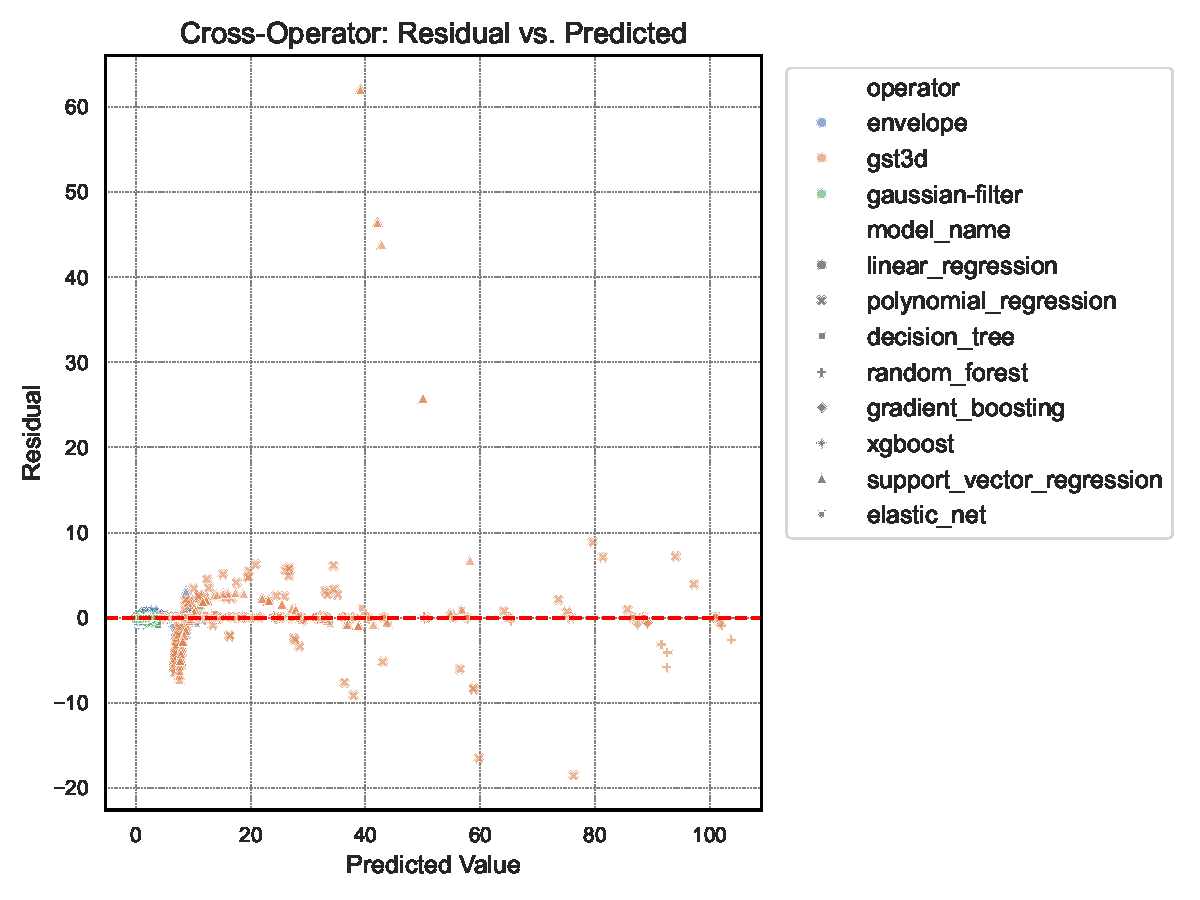
\includegraphics[width=\textwidth]{assets/images/05/residual_vs_predicted}
        \caption{Residual vs. predicted values (\ac{GB})}
    \end{subfigure}
    \hfill
    \begin{subfigure}[t]{0.49\textwidth}
        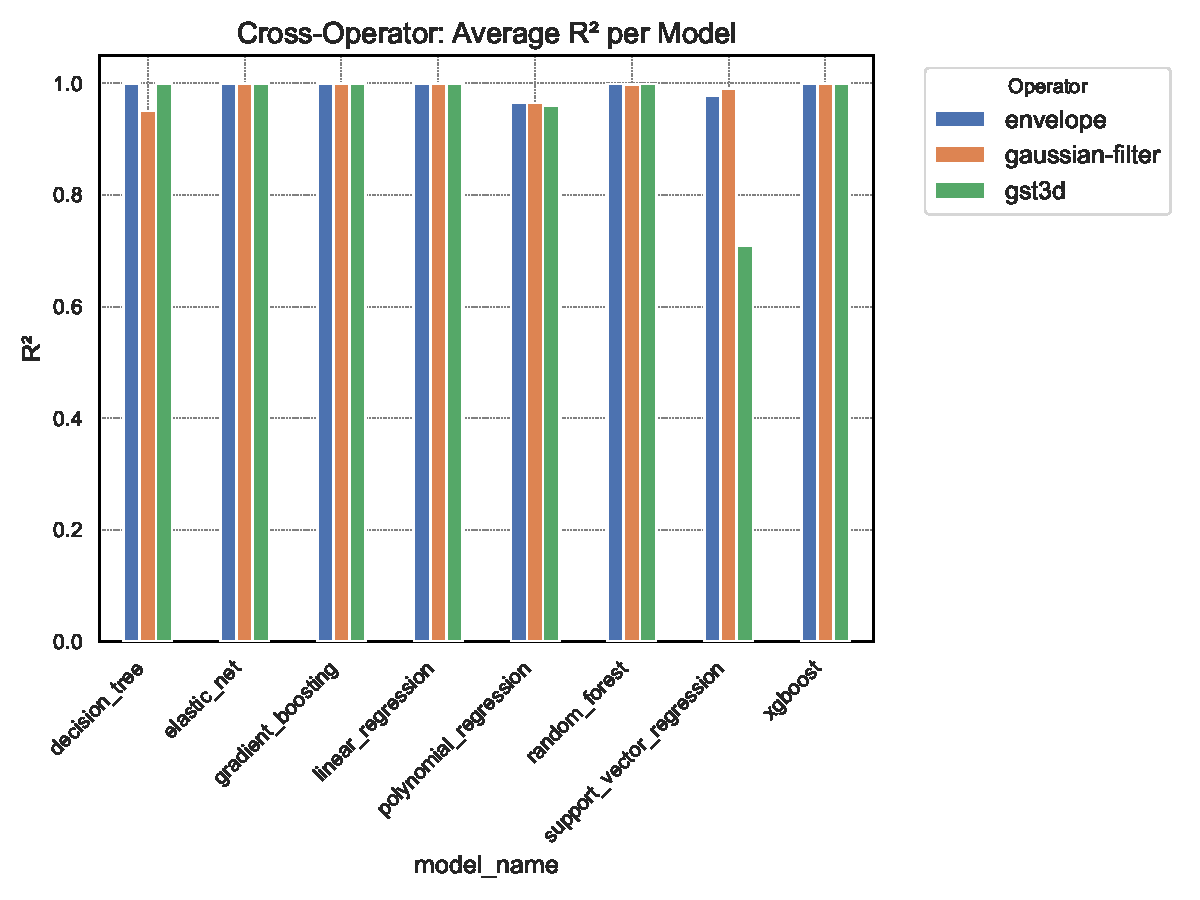
\includegraphics[width=\textwidth]{assets/images/05/cross_model_r2_bar}
        \caption{$R^2$ scores}
    \end{subfigure}
    \caption{Cross‐model, cross‐operator prediction performance:
        (a) Scatter of residuals versus predicted peak memory (\ac{GB}) for each regression model and operator, with the dashed red line at zero highlighting bias and outliers.
        (b) Mean $R^2$ scores for each model, averaged across Envelope, \ac{GST3D}, and Gaussian Filter—demonstrating that simple linear approaches (Linear Regression, Elastic Net) achieve near‐perfect explanatory power, with more complex models providing negligible gains.}
    \label{fig:residual_vs_predicted_and_r2_bar}
\end{figure*}

Table~\ref{tab:performance_summary} highlights the best-performing model per operator.

\begin{table}[htbp]
    \centering
    \begin{tabular}{lccc}
        \hline
        \textbf{Operator} & \textbf{Best Model} & \textbf{Score} & \textbf{Note}                   \\
        \hline
        Envelope          & Linear Regression   & 2.900          & Edges out Elastic Net           \\
        \ac{GST3D}        & Linear Regression   & 2.349          & Top $R^2$, low residuals        \\
        Gaussian Filter   & Elastic Net         & 2.990          & Just ahead of Linear Regression \\
        \hline
    \end{tabular}
    \caption{Updated top models and scores from the new \ac{CSV} data.}
    \label{tab:performance_summary}
\end{table}

Figures~\cref{fig:actual_vs_predicted_envelope,fig:actual_vs_predicted_gst3d,fig:actual_vs_predicted_gaussian} confirm that these models closely align with actual memory values.

\begin{figure}[htbp]
    \centering
    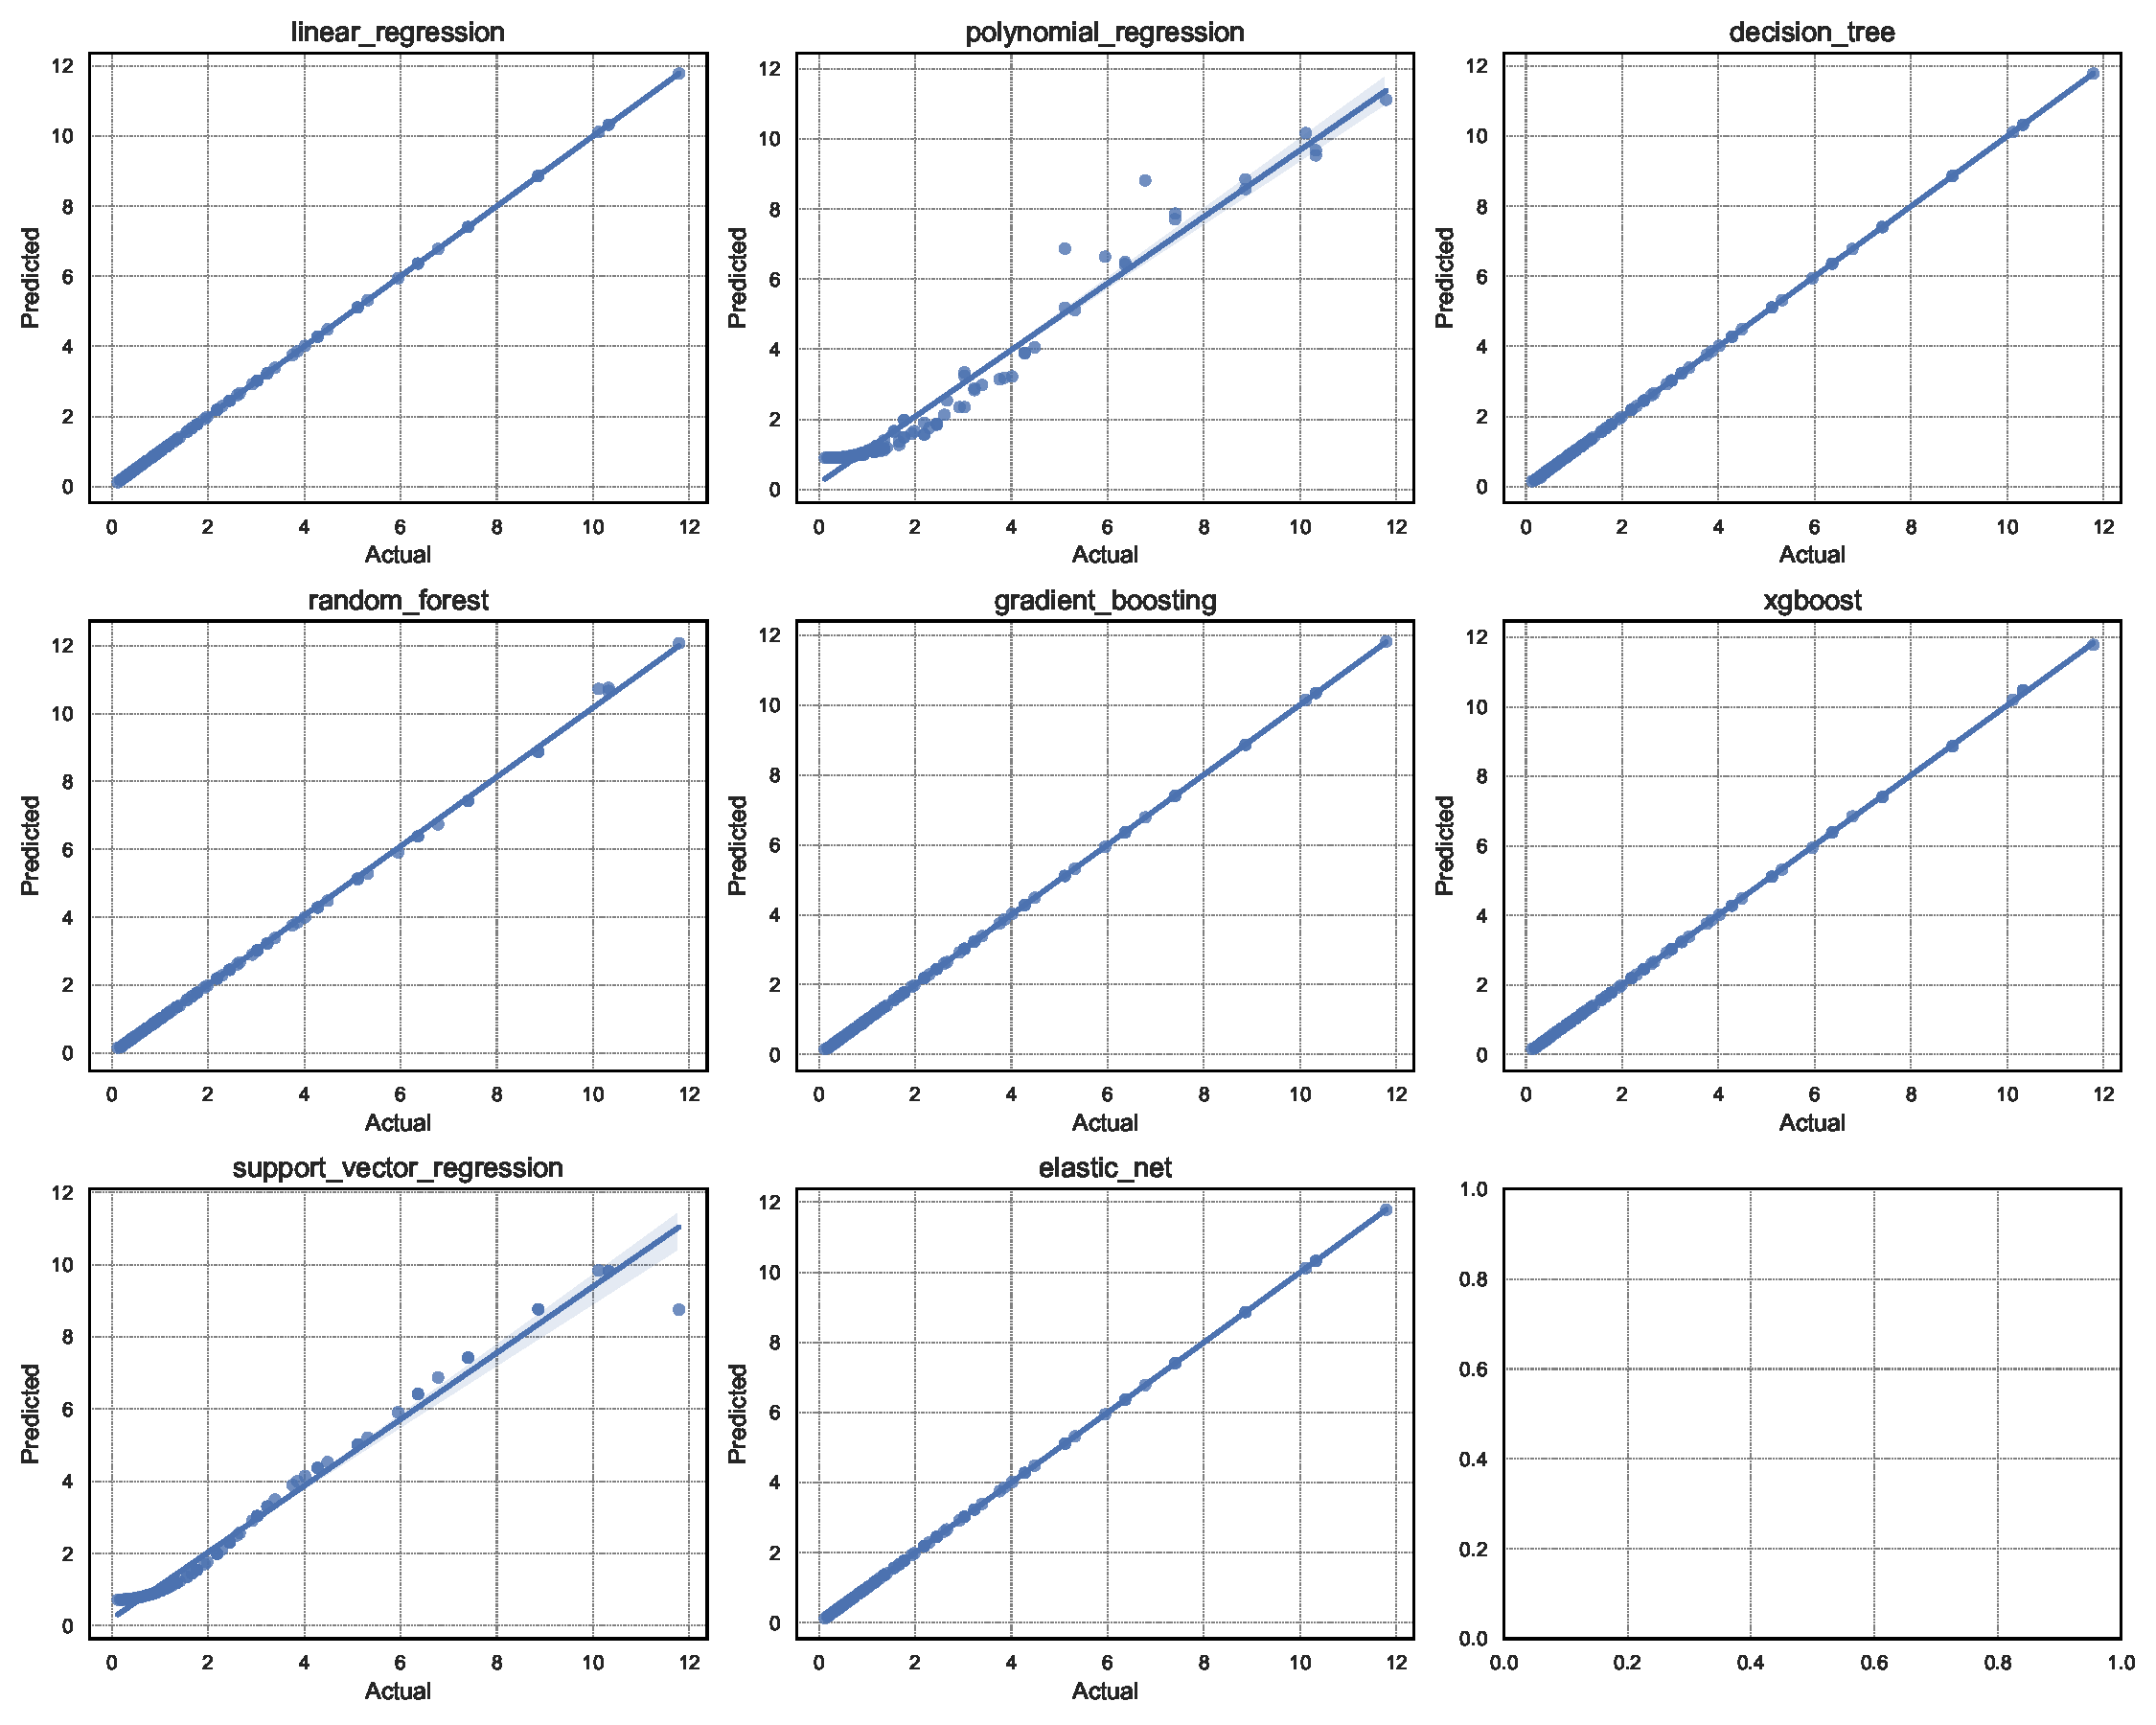
\includegraphics[width=\textwidth]{assets/images/05/actual_vs_predicted_by_model_envelope}
    \caption{Predicted vs.\ actual peak memory usage (\ac{GB}) for Envelope across eight regression models (Linear Regression, Polynomial Regression, Decision Tree, Random Forest, Gradient Boosting, \ac{XGBoost}, Support Vector Regression, Elastic Net). Each scatter plot includes the identity line ($y=x$), demonstrating near‐perfect alignment for most models and slight over-/underestimation at the high end for Polynomial Regression and \ac{SVR}.}
    \label{fig:actual_vs_predicted_envelope}
\end{figure}
\clearpage

\begin{figure}[htbp]
    \centering
    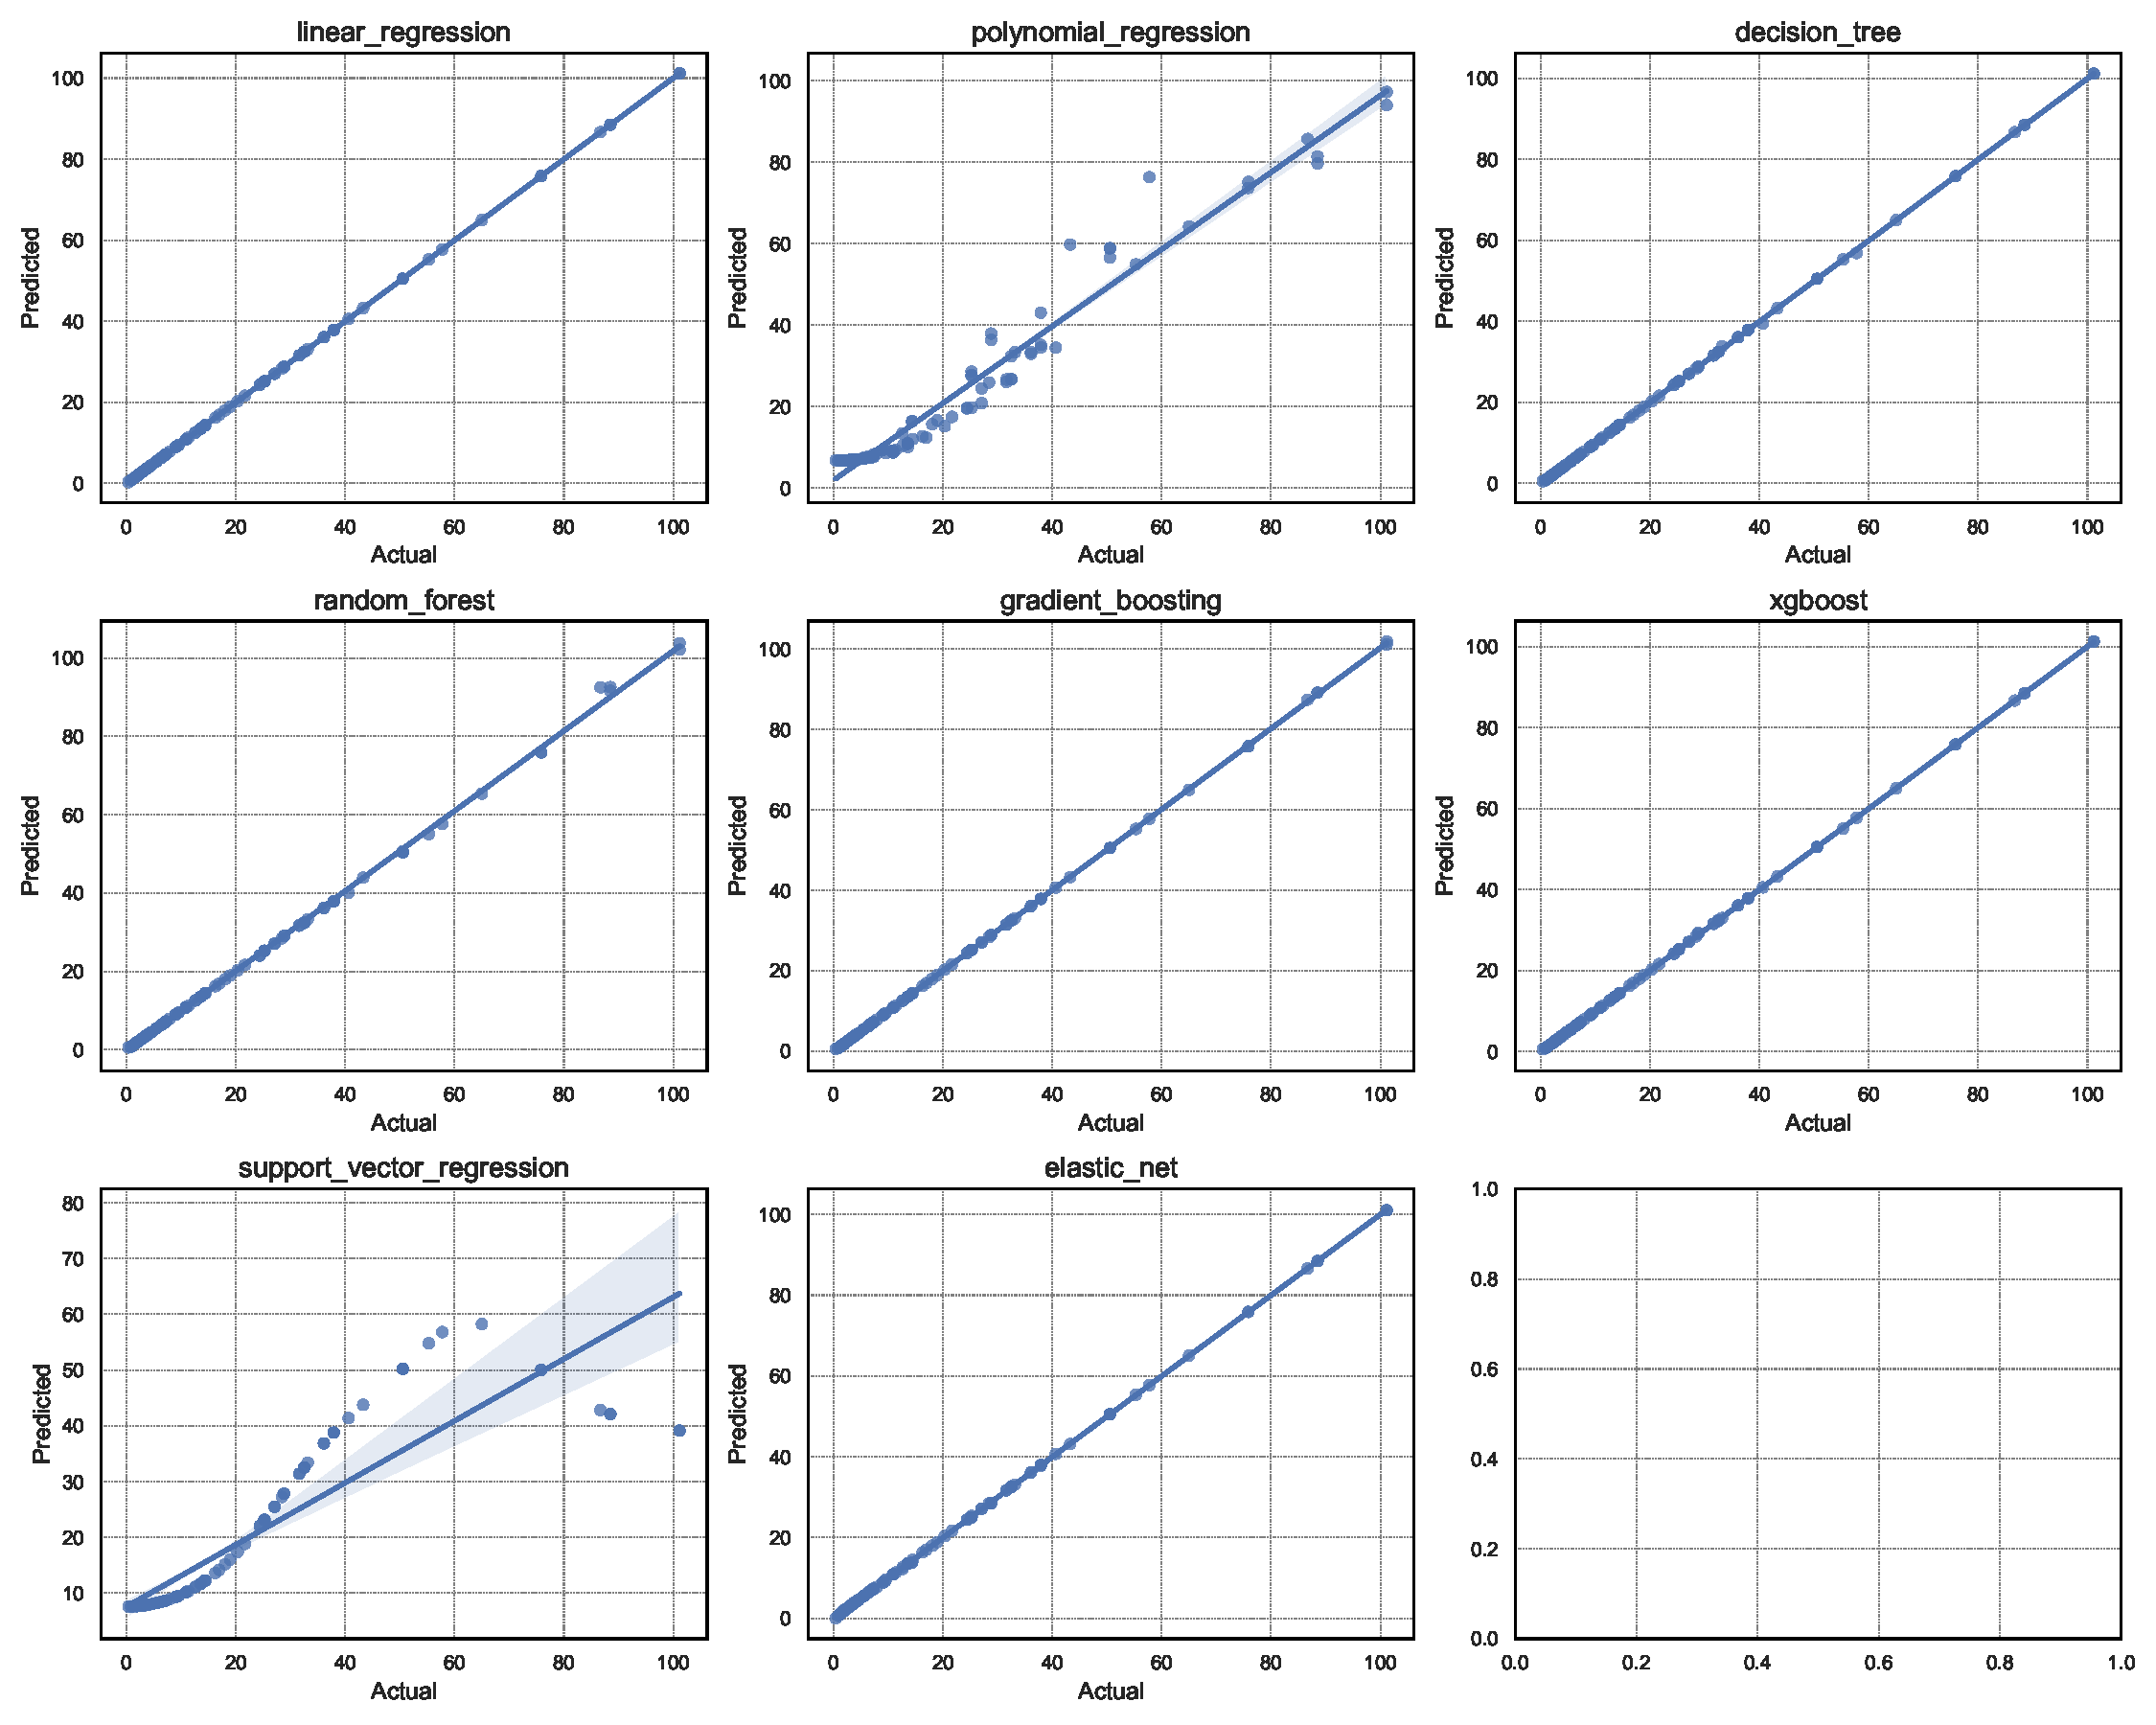
\includegraphics[width=\textwidth]{assets/images/05/actual_vs_predicted_by_model_gst3d}
    \caption{Predicted vs.\ actual peak memory usage (\ac{GB}) for \ac{GST3D} across the same eight regression models. All models closely follow the ideal $y=x$ line, with small deviations in Polynomial Regression and \ac{SVR} visible at mid‐range volumes.}
    \label{fig:actual_vs_predicted_gst3d}
\end{figure}
\clearpage

\begin{figure}[htbp]
    \centering
    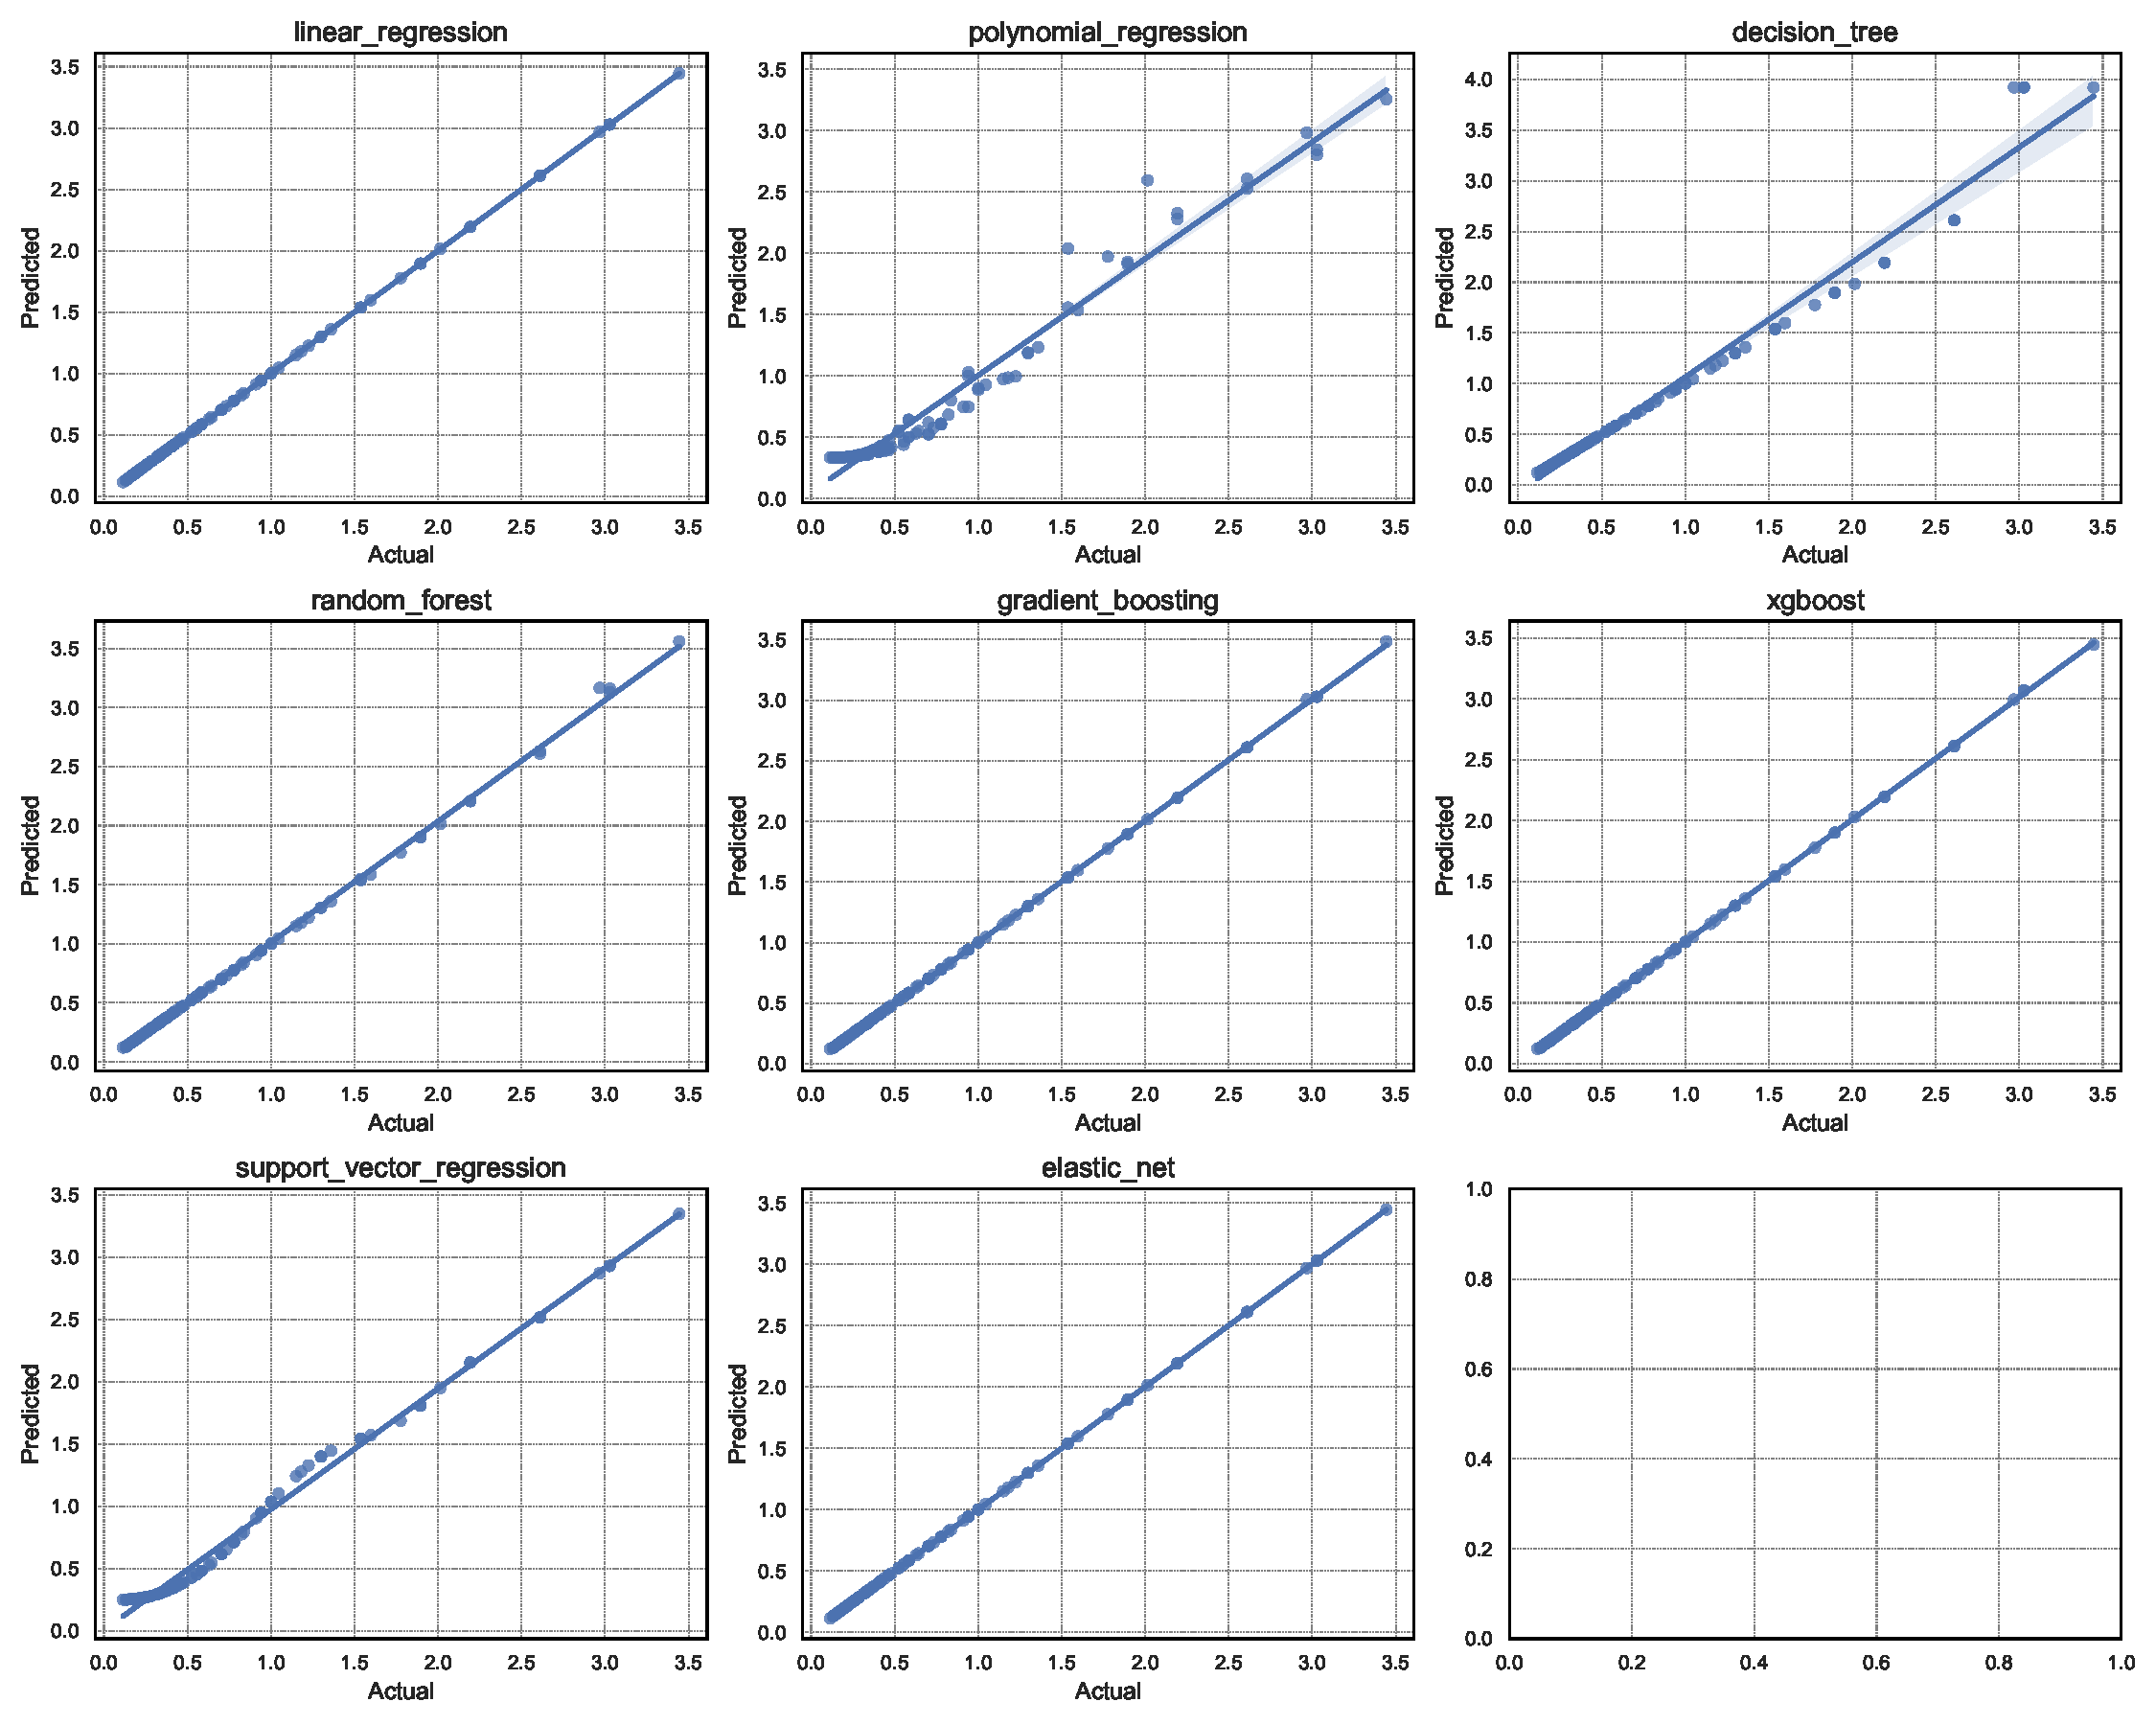
\includegraphics[width=\textwidth]{assets/images/05/actual_vs_predicted_by_model_gaussian-filter}
    \caption{Predicted vs.\ actual peak memory usage (\ac{GB}) for Gaussian Filter using eight regression models. Linear Regression, Elastic Net, Random Forest, Gradient Boosting, and \ac{XGBoost} exhibit almost perfect predictions, while Polynomial Regression and \ac{SVR} show minor bias at the smallest and largest values.}
    \label{fig:actual_vs_predicted_gaussian}
\end{figure}
